\documentclass[11pt,a4paper]{article}
\usepackage[margin=2.3cm]{geometry}
\usepackage{amsmath,amssymb,booktabs,array,xcolor,microtype,float,tikz}
\usepackage[colorlinks,linkcolor=blue!50!black,urlcolor=blue!60!black]{hyperref}
\setlength{\parskip}{0.5em}
\setlength{\parindent}{0pt}
\newcommand{\dd}{\mathrm{d}}
\newcommand{\code}[1]{\texttt{\small #1}}

\title{\textbf{What the LO fast grid computes}}
\author{Notes on \code{fastgrid\_codes/sf\_lo\_\{L,T\}\_fastgrid.py}}
\date{2 October 2026}

\begin{document}
\maketitle

\noindent\fbox{\parbox{0.97\linewidth}{
\textbf{In one sentence.} The \code{make} mode still does the $z$-integral at fixed $r$, exactly as before; it then turns those values into one number $w_n$ per node $r_n$ of the dipole table, so that the \code{use} mode is the dot product $F=\sum_n w_n\,N(r_n,Y)$ of the weights with one row of the table.}}

\section{The integral to be computed}
With $u=\ln r$, the LO structure functions are a single integral over the dipole size,
\begin{equation}
\label{eq:F}
F_{L,T}(x,Q^2)=\int\dd u\;G_{L,T}(u)\,N(u,Y),\qquad Y=\ln\frac{x_0}{x},
\end{equation}
where all the dependence on the photon is in the kernel $G$, which is the \textbf{$z$-integral at fixed $r$}:
\begin{align}
G_L(u)&=\sum_f\frac{2N_cQ^4e_f^2}{\pi^3}\,r^2\!\int_0^1\!\dd z\;z^2(1-z)^2K_0^2(\epsilon_f r),\\
G_T(u)&=\sum_f\frac{N_cQ^2e_f^2}{2\pi^3}\,r^2\!\int_0^1\!\dd z\;\Big\{[z^2+(1-z)^2]\epsilon_f^2K_1^2(\epsilon_f r)+m_f^2K_0^2(\epsilon_f r)\Big\},
\end{align}
with $r=e^u$, $\epsilon_f^2=z(1-z)Q^2+m_f^2$ and a factor $\sigma_0/2$ left out. One factor $r$ comes from $\dd^2r=2\pi r\,\dd r$ and the other from $\dd r=r\,\dd u$. $G$ depends on $Q^2$ but not on $x$ or on the dipole; that is what makes a fast grid possible. In the code, $G$ at a given $r$ is \code{prefactor * r**2 * z\_integral\_\{L,T\}(r, ...)}.

\section{What we know about the dipole}
The dipole is only known at the nodes of its table, which are uniformly spaced in $u$:
\begin{equation}
u_n=\ln r_{\min}+n\,h,\qquad h=\ln(\mathrm{mult}),\qquad N_n(Y)\equiv N(u_n,Y),\qquad n=0,\dots,n_r-1 .
\end{equation}
Between the nodes, the Julia and Python reference codes (\code{sf\_lo\_\{L,T\}.jl}, \code{sf\_lo\_\{L,T\}.py}) interpolate linearly in $u$. That interpolant can be written with the ``hat'' functions $\phi_n$ of Fig.~\ref{fig:hat}:
\begin{equation}
\label{eq:hat}
N(u,Y)=\sum_n N_n(Y)\,\phi_n(u),\qquad \phi_n(u)=\max\Big(0,\;1-\frac{|u-u_n|}{h}\Big).
\end{equation}
Each $\phi_n$ is 1 at its own node, 0 at all other nodes, and linear in between.

\begin{figure}[H]
\centering
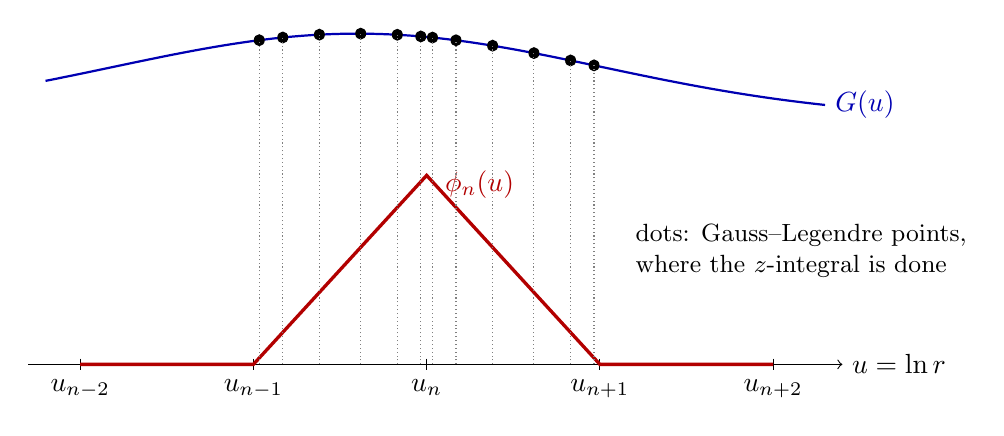
\begin{tikzpicture}[xscale=2.2,yscale=2.4]
\draw[->] (-0.3,0) -- (4.4,0) node[right] {$u=\ln r$};
\foreach \i/\lab in {0/{u_{n-2}},1/{u_{n-1}},2/{u_n},3/{u_{n+1}},4/{u_{n+2}}} {
  \draw (\i,0.03) -- (\i,-0.03) node[below] {$\lab$};
}
% G(u)
\draw[thick,blue!70!black,domain=-0.2:4.3,samples=80] plot (\x,{1.3+0.45*exp(-0.25*(\x-1.6)*(\x-1.6))}) node[right] {$G(u)$};
% hat function of node n
\draw[very thick,red!70!black] (0,0) -- (1,0) -- (2,1) -- (3,0) -- (4,0);
\node[red!70!black,right] at (2.05,0.95) {$\phi_n(u)$};
% Gauss-Legendre points in the two intervals of the hat
\foreach \a in {1,2} {
  \foreach \t in {-0.9325,-0.6612,-0.2386,0.2386,0.6612,0.9325} {
    \pgfmathsetmacro{\xx}{\a+0.5+0.5*\t}
    \pgfmathsetmacro{\yy}{1.3+0.45*exp(-0.25*(\xx-1.6)*(\xx-1.6))}
    \fill[black] (\xx,\yy) circle (0.9pt);
    \draw[gray,densely dotted] (\xx,0) -- (\xx,\yy);
  }
}
\node[align=left,font=\small,right] at (3.15,0.6) {dots: Gauss--Legendre points,\\where the $z$-integral is done};
\end{tikzpicture}
\caption{Uniform grid in $u=\ln r$ (the dipole table's own nodes), the hat function $\phi_n$ of node $n$, and the kernel $G(u)$. The weight $w_n$ is the area under $G\,\phi_n$; it is computed from $G$ at the marked points in the two intervals next to $u_n$.}
\label{fig:hat}
\end{figure}

\section{From the integral to a dot product}
Inserting Eq.~\eqref{eq:hat} into Eq.~\eqref{eq:F} gives
\begin{equation}
\label{eq:dot}
\boxed{F(x,Q^2)=\sum_n w_n\,N_n(Y),\qquad w_n=\int\dd u\;G(u)\,\phi_n(u)}
\end{equation}
This is exact for the linearly interpolated dipole: no further approximation is made. The weights $w_n$ live on exactly the dipole's grid and do not depend on $x$ or on the dipole, so
\begin{itemize}
\item \code{make} computes the vector $(w_0,\dots,w_{n_r-1})$ once per $Q^2$ (and polarisation) and writes it to the grid file, one row per node;
\item \code{use} reads one row of the dipole table, $N_n(Y)$, and returns $\sum_n w_nN_n(Y)$. If $Y=\ln(x_0/x)$ falls between two table rows, the row is first interpolated linearly in $Y$, as in the reference codes; if it falls on a row, it is literally that row.
\end{itemize}

\section{Where the \texorpdfstring{$z$}{z}-integral at fixed \texorpdfstring{$r$}{r} comes in}
Written out, the weight is a weighted average of $G$ over the two intervals next to the node:
\begin{equation}
w_n=\int_{u_{n-1}}^{u_n}\dd u\;G(u)\,\frac{u-u_{n-1}}{h}\;+\;\int_{u_n}^{u_{n+1}}\dd u\;G(u)\,\frac{u_{n+1}-u}{h}.
\end{equation}
These are ordinary one-dimensional integrals over $u$ of a smooth function. \code{make} evaluates them with a 6-point Gauss--Legendre rule on each interval $[u_k,u_{k+1}]$ (exact for polynomials up to degree 11):
\begin{equation}
\int_{u_k}^{u_{k+1}}\dd u\,f(u)\simeq\frac h2\sum_{j=1}^6\omega_j\,f\Big(u_k+\tfrac h2(1+t_j)\Big),
\end{equation}
with $t_j,\omega_j$ the Legendre nodes and weights. \textbf{Every evaluation of $G$ at such a point is the $z$-integral at fixed $r=e^u$}, done by SciPy's \code{quad} exactly as before. So the $z$-integral at fixed $r$ is still the basic step; it is just done at six values of $r$ inside each node interval rather than only at the nodes, and the results are then combined into one number per node. Gauss--Legendre is only the rule for the $u$-integral that builds $w_n$; it does not change the grid, which is the dipole's.

To lowest order $w_n\simeq h\,G(u_n)$, since $\int\phi_n\,\dd u=h$. The difference from $h\,G(u_n)$ accounts for how $G$ varies across the hat.

\textbf{Ends of the grid.} Below the first node the dipole is taken to be zero. If the upper limit \code{--rmax} lies beyond the last node, the dipole is held at its last value there, as in the reference codes, and that tail is added to the last weight. If \code{--rmax} lies inside the grid, only the part of each hat below it is integrated.

\section{The three ways of building the weights}
All three give $F$ as a sum over grid points; they differ in which $r$ values $G$ is evaluated at and in what is assumed about the dipole between its nodes.

\begin{table}[H]
\centering\small
\renewcommand{\arraystretch}{1.35}
\begin{tabular}{@{}p{3.2cm} p{3.6cm} p{3.4cm} p{4.6cm}@{}}
\toprule
& $G$ evaluated at & \code{use} step & Accuracy\\
\midrule
(a) Previous version: fine Simpson grid & 2001 points uniform in $u$, independent of the dipole & interpolate $N$ onto the fine grid, then Simpson sum & error from the kinks of the linear interpolant at the table nodes; needed spacing $\ll h$; error $\sim10^{-6}$ at 2001 points\\
(b) Node quadrature: $w_n=s_n\,h\,G(u_n)$ & the nodes only & dot product with the table row & $\mathcal O(h^4)$ for a \emph{smooth} dipole through the nodes, but differs from the linear-interpolation result by $\mathcal O(h^2)$\\
(c) \textbf{Current}: hat weights, Eq.~\eqref{eq:dot} & 6 Gauss--Legendre points per node interval & dot product with the table row & exact for the linearly interpolated dipole; matches the reference codes\\
\bottomrule
\end{tabular}
\end{table}
Here $s_n$ are quadrature weights, for example the extended Simpson weights that \code{BK\_evolve\_tf.py} uses,
\[
(s_0,s_1,s_2,s_3,\dots,s_{n_r-1})=(9,\,28,\,23,\,24,\,\dots,\,24,\,23,\,28,\,9)/24 .
\]

Options (b) and (c) disagree by the error of linear interpolation itself, which is of order $h^2N''$. Your BK solver documents this effect: \code{BK\_evolve\_tf.py} switched to cubic splines because linear interpolation of the convex $N(\ln r)$ biased every evaluation high by about $+0.08\%$ on its grid. So the choice between (b) and (c) is a choice of what the dipole is between its nodes:
\begin{itemize}
\item (c) reproduces the Julia and Python reference codes, which interpolate linearly;
\item (b) treats the tabulated dipole as samples of a smooth function, as your BK solver does internally, and needs $G$ only at the nodes.
\end{itemize}
Both give a dot product with a row of the table on the same uniform grid. Switching from (c) to (b) is a small change in \code{make}.

\section{Checks of the current version}
\begin{itemize}
\item Against a direct high-precision integral of $G$ times the linearly interpolated dipole (adaptive, interval by interval, relative tolerance $10^{-11}$), for \code{median\_bk} at $Q^2=10$~GeV$^2$, $x=10^{-3}$, $r\le20$~GeV$^{-1}$: agreement to $2\times10^{-12}$ ($F_L$) and $3\times10^{-13}$ ($F_T$).
\item Against the Julia reference codes at six points (both polarisations, both dipole tables, $Q^2=2$ to $27$~GeV$^2$, with and without charm), using \code{--rmax 20} to match their \code{xmax}: agreement to $7.4\times10^{-6}$ ($1.2\times10^{-5}$ for one charm part), which is the Julia codes' own quadrature tolerance of $10^{-5}$.
\end{itemize}

\end{document}
